\documentclass[12pt]{article}
\usepackage[utf8]{inputenc}
\usepackage{cite} % cite{label}
\usepackage{amsmath} % bmatrix
\usepackage[pdftex]{graphicx}
\usepackage{adjustbox}

\usepackage{algorithm}% For algorithm table
\usepackage{algpseudocode}% For algorithm table

\begin{document}

\title{Estimating 3D Structure from Motion using\\
the Normalized Eight Point Algorithm\\
and LUP Decomposition\\}
\author{Alexander Koumis\\
Computer Engineering Department\\
San Jose State University\\
me@alexander.computer}
\date{November 2014}
\maketitle

\begin{abstract}
This paper examines the Eight-point algorithm, which computes a Fundamental matrix from a pair of feature sets extracted from two images of the same scene. The RANSAC scheme is then used to remove outliers by performing the algorithm repeatedly on the point sets, removing those which fall beneath a set threshold.
\end{abstract}

\newpage

\section{Introduction}
Recently published work regarding 3D reconstruction~\cite{Hartley2004} presents new market opportunities in the areas of surveillance, autonomous vehicle networks, augmented reality, and more. SfM (Structure from Motion), or obtaining a 3D representation of a physical object based on an image set of said objects, provides a wealth of information for such aforementioned fields, giving robotic systems a better understanding of the world around them. Photogrammetric methods of capturing 3D representations of scenes and objects are also compellingly cheaper than their laser-based (LIDAR) alternatives.
In this work, the \textit{Normalized eight-point algorithm} is examined as a means of extracting the Fundamental matrix, used to estimate 3D coordinates based on 2D parameters.

\section{Background and Objectives}
Modern photogrammetry-influenced SfM pipelines have several options for computing estimated 3D world points from a pair of 2D features, extracted from two images. Most SfM algorithms involve computation of $F$, the Fundamental Matrix, introduced by Q. T. Luong~\cite{AICPub329:1992}, a parametrized way to describe the 3D relationship between a pair of feature matches, satisfying homogeneous equation~\eqref{eq:fundamental}~\cite{Hartley2004}. This paper aims to provide a verbose walkthrough of one particular pipeline for computing $F$, as well as using $F$ to determine the coordinates of the 3D world points. This method follows closely the implementation provided by the open-source SfM software package \textit{Bundler}~\cite{NoahSnavely}.

\section{Findings and Analysis}
$x$ and $x'$ are determined by extracting keypoints and/or descriptors from two images, using any number of algorithms, such as SIFT~\cite{Lowe:2004:DIF:993451.996342}, SURF~\cite{Bay:2008:SRF:1370312.1370556},  using sets extracted from 2D images, the column-extended 2D feature coordinates (equation \eqref{eq:points}) with all $z$ values in $x$ and $x'$ set to 1).

\begin{center}
    \begin{equation}\label{eq:fundamental}
        {x}'^TFx = 0
    \end{equation}
\end{center}


\begin{align}\label{eq:points}
    x = 
    \begin{bmatrix}
        x_1 & y_1 & z_1\\ 
        x_2 & y_2 & z_2\\ 
        \vdots&\vdots&\vdots\\ 
        x_n&y_n&z_n\\
    \end{bmatrix}
    &&
    x` =
    \begin{bmatrix}
        x`_1 & y`_1 & z`_1\\ 
        x`_2 & y`_2 & z`_2\\ 
        \vdots & \vdots & \vdots\\ 
        x`_n&y`_n&z`_n\\
    \end{bmatrix}
\end{align}

\subsection{Eight point algorithm}
The eight point algorithm, introduced by Longuet-Higgens in 1987 ~\cite{Longuet-Higgins:1987:CAR:33517.33523}, assumes the left hand side of equation~\eqref{eq:fundamental} as a singular value, equals to zero with 9 unknowns, which can therefore be solved with 8 linearly independent vectors. Rearranging equation~\eqref{eq:fundamental} by multiplying both sides by ${x}^-1$ allows the problem to be expressed as equation~\eqref{eq:Af}, where $A$ is defined as the $n\times9$ cross product of each match pair in $x$ and $x'$.

As the measurements are typically noisy, the solution must be calculated as a least squares minimization, where $||f||=1$, achievable by setting $F_{33}$ to 1. With $z_i$  and $z'_i$ also both equals to 1, $A$ becomes a square 8x8 matrix (see equation~\eqref{eq:expanded8Pt}, accurate to scale (projective accuracy rather than Euclidean), allowing $F$ to be solved using one of several linear solvers. LU decomposition with partial row pivoting is explored in this paper.

\begin{equation}\label{eq:Af}Af=0\end{equation}

\begin{align}\label{eq:fullFundamental}
    \resizebox{0.5\textwidth}{!}{
        $\begin{bmatrix}
            x_1x_1' & y_1x_1' & z_1x_1' & x_1y_1' & y_1y_1' & z_1y_1' & x_1z_1' & y_1z_1' & z_1z_1'\\
            \vdots&\vdots&\vdots&\vdots&\vdots&\vdots&\vdots&\vdots&\vdots\\
            x_nx_n' & y_nx_n' & z_nx_n' & x_ny_n' & y_ny_n' & z_ny_n' & x_nz_n' & y_nz_n' & z_nz_n'\\
        \end{bmatrix}
        \begin{bmatrix}
            F_{11}\\F_{12}\\F_{13}\\F_{21}\\F_{22}\\F_{23}\\F_{31}\\F_{32}\\F_{33}
        \end{bmatrix}$
        =0
    }
\end{align}

\begin{align}\label{eq:expanded8Pt}
    \resizebox{0.5\textwidth}{!}{
        $\begin{bmatrix}
            x_1x_1' & y_1x_1' & x_1' & x_1y_1' & y_1y_1' & y_1' & x_1 & y_1\\
            x_2x_2' & y_2x_2' & x_2' & x_2y_2' & y_2y_2' & y_2' & x_2 & y_2\\
            x_3x_3' & y_3x_3' & x_3' & x_3y_3' & y_3y_3' & y_3' & x_3 & y_3\\
            x_4x_4' & y_4x_4' & x_4' & x_4y_4' & y_4y_4' & y_4' & x_4 & y_4\\
            x_5x_5' & y_5x_5' & x_5' & x_5y_5' & y_5y_5' & y_5' & x_5 & y_5\\
            x_6x_6' & y_6x_6' & x_6' & x_6y_6' & y_6y_6' & y_6' & x_6 & y_6\\
            x_7x_7' & y_7x_7' & x_7' & x_7y_7' & y_7y_7' & y_7' & x_7 & y_7\\
            x_8x_8' & y_8x_8' & x_8' & x_8y_8' & y_8y_8' & y_8' & x_8 & y_8
        \end{bmatrix}
        \begin{bmatrix}
            F_{11}\\F_{12}\\F_{13}\\F_{21}\\F_{22}\\F_{23}\\F_{31}\\F_{32}
        \end{bmatrix}$
        =0
    }
\end{align}

\subsection{Normalized eight point algorithm}

The traditional eight point algorithm has been criticized for producing inaccurate results, given the aforementioned presence of inevitably noisy measurements.  Hartley’s 1997 ~\cite{Hartley:1997:DEA:262631.262634} defense of the eight point algorithm states the algorithm is fundamentally sound in theory, and simply needs normalization of its input parameters to produce more robust results. The errors, he suggests, stem from the fact that the arbitrary $1$ chosen for the third dimension of $x$ and $x`$ are not normalized with respects to the first and second dimensions.
His solution comes in form of the \textit{Normalized eight point algorithm}, which first computes the centroid for both sets of points, or the normalized average of the values in each dimension:

\begin{align}\label{eq:centroid}
    c =\begin{bmatrix}
        \frac{\sum_{i}^{8}x_i}{8\sqrt{2}} & \frac{\sum_{i}^{8}y_i}{8\sqrt{2}} & \frac{\sum_{i}^{8}z_i}{8\sqrt{2}}
    \end{bmatrix}
&&
    c' =\begin{bmatrix}
        \frac{\sum_{i}^{8}x'_i}{8\sqrt{2}} & \frac{\sum_{i}^{8}y'_i}{8\sqrt{2}} & \frac{\sum_{i}^{8}z'_i}{8\sqrt{2}}
    \end{bmatrix}
\end{align}

The average distance from each point sets' centroid is calculated, by finding the average magnitude of difference between each point's coordinate and the centroid:

\begin{align}\label{eq:avgDistance}
    dist = \frac{
        \sum_{i}^{8}
        \sqrt{x_i^{2}+y_i^{2}+z_i^{2}}
    }{8}
&&
    dist' = \frac{
        \sum_{i}^{8}
        \sqrt{x`_i^{2}+y`_i^{2}+z`_i^{2}}
    }{8}
\end{align}

The points are then scaled by the inverse of the average distance, which are then plugged into equation ~\eqref{eq:expanded8Pt}:

\begin{align}\label{eq:scale}
    scale = \frac{1}{dist}
&&
    scale' = \frac{1}{dist'}
\end{align}

\begin{align}\label{eq:pointsScaled}
    x = \begin{bmatrix}
        \frac{x_1}{scale} & \frac{y_1}{scale} & \frac{z_1}{scale}\\[0.3em]
        \frac{x_2}{scale} & \frac{y_2}{scale} & \frac{z_2}{scale}\\[0.3em]
        \vdots & \vdots & \vdots\\ 
        \frac{x_n}{scale} & \frac{y_n}{scale} & \frac{z_n}{scale}\\[0.3em]
    \end{bmatrix}
&&
    x' =
    \begin{bmatrix}
        \frac{x'_1}{scale'} & \frac{y'_1}{scale'} & \frac{z'_1}{scale'}\\[0.3em] 
        \frac{x'_2}{scale'} & \frac{y'_2}{scale'} & \frac{z'_2}{scale'}\\[0.3em]
        \vdots & \vdots & \vdots\\ 
        \frac{x'_n}{scale'} & \frac{y'_n}{scale'} & \frac{z'_n}{scale'}\\[0.3em]
    \end{bmatrix}
\end{align}
\\
The scaled points are then plugged into equation~\eqref{eq:expanded8Pt}, which is solved using $LUP$ decomposition. $F$ is then de-normalized by transforming the scaled coordinates back to the original for further use.

\subsection{LUP Decomposition with Partial Row Pivoting}
A brief primer on LUP Decomposition is presentented as a means of solving equation~\eqref{eq:expanded8Pt}.

LUP decomposition with partial row pivoting breaks up the problem into a higher (upper) and lower matrix, as well as a permutation matrix, which initially set to the identity matrix, keeps track of row switches:

\begin{equation}
    PA=LU
\end{equation}

To ensure the solution spans all 8 column vectors, $A$ is solved by zeroing out the $ith$ column (below $A_{ij}$), where $i = 1 ... 8$, placing the resulting values in $U$ and the coefficient used to make the element 0. For every diagonal entry $A_{ij}$, each value in the row $i+1$ is subtracted by $\frac{A_{ij+1}}{A_{ij}}$ multiplied by the corresponding row value.

After the process is complete, the solution $F$ is determined using back and forward substitution on the upper triangular $U$. 

\subsection{Triangulation}
After $F$ has been determined, the constraints equation describing the relationship between $x$ and $x'$, $X$ (estimated 3D points), and projection (camera) matrices $P$ and $P'$ can be expressed as:

\begin{align}\label{eq:xPX}
    x=PX
&&
    x'=P'X
\end{align}

The first projection matrice assumes the canonical projection $\begin{matrix}P=[I|0]\end{matrix}$, with $\begin{matrix}P'=[R|t]\end{matrix}$, allowing the equations from equation~\eqref{eq:xPX} to be expanded as the following homogeneous equations ($R$ and $t$ being the $3x3$ \textit{rotation matrix} and \textit{translation vector}, respectively):

\begin{equation}\label{eq:xPX_expanded}
    \begin{bmatrix}
        x\\
        y\\
        z
    \end{bmatrix}
    =
    \begin{bmatrix}
        1 & 0 & 0 & 0\\
        0 & 1 & 0 & 0\\
        0 & 0 & 1 & 0
    \end{bmatrix}
    \begin{bmatrix}
        X\\
        Y\\
        Z\\
        W\\
    \end{bmatrix}
\end{equation}
\begin{equation}\label{eq:x'P'X_expanded}
    \begin{bmatrix}
        x'\\
        y'\\
        z'
    \end{bmatrix}
    =
    \begin{bmatrix}
        R_{11} & R_{12} & R_{13} & t_1\\
        R_{21} & R_{22} & R_{23} & t_2\\
        R_{31} & R_{31} & R_{33} & t_3
    \end{bmatrix}
    \begin{bmatrix}
        X\\
        Y\\
        Z\\
        W\\
    \end{bmatrix}
\end{equation}

\begin{figure}\begin{center}
    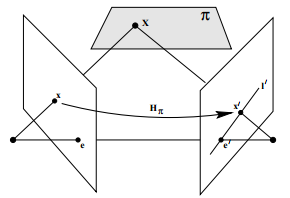
\includegraphics[scale=0.6]{images/homography.png}
        \caption{Estimating 3D feature coordinate from 2D features ~\cite{Hartley2004}}
        \label{fig:homography}
\end{center}\end{figure}

Assuming the pinhole camera model, with $P'=K[R|t]$ ~\cite{moulon:hal-00829332} (discussion of $K$, the camera intrinsics matrix, omit), $R$ is compute as the cross product of $\textbf{e'}$ and $F$, $\textbf{e'}$ defined as the second image projection's \textit{epipole}, or the position of the projection of the first camera's centroid on the second image (see figure \ref{fig:homography}):

\begin{equation}\label{eq:P_prime}
    P'=
    \begin{bmatrix}
        [\mathbf{e'}]_\times F|\mathbf{e'}
    \end{bmatrix}
\end{equation}

One of the properties of the fundamental matrix is that if calculated for the projection matrice pair $(P, P')$, it holds that $F^{T}$ is the fundamental matrix for the pair $(P', P)$.

$l$ and $l'$, the \textit{epipolar} lines between the feature point and each image's epipole, are defined as the following (and illustrated in figure~\ref{fig:epipolar}):

\begin{align}\label{eq:epipolarLines}
    l = Fx
&&
    l' = F^Tx'
\end{align}

It is clear from figure~\ref{fig:homography} that $\textbf{e}$ and $\textbf{e'}$ always lie upon $l$ and $l'$, allowing for $e'$ to be expressed as the \textit{right null-space} of $F$, now easily solvable with Gaussian elimination or Cramer's rule: 

\begin{equation}\label{eq:F_left_nullspace}
    \textbf{e'}^TF=0
\end{equation}

\begin{figure}\begin{center}
    \includegraphics[scale=0.6]{images/epipolar.png}
        \caption{Epipolar geometry ~\cite{Hartley2004}}
        \label{fig:epipolar}
\end{center}\end{figure}

Once $\textbf{e'}$ has been determined, $P'$ can be found by substituting the found $\textbf{e'}$ and $F$ values into equation ~\eqref{eq:P_prime}, expanded as follows:

\begin{equation}
        P'=
    \begin{bmatrix}
        \begin{bmatrix}
             0      & -e'^{3} &  e'^{2}\\
             e'^{3} &  0      & -e'^{1}\\
            -e'^{2} &  e'^{1} &  0
        \end{bmatrix}
        \begin{bmatrix}
            F_{11} & F_{12} & F_{13}\\
            F_{21} & F_{22} & F_{23}\\
            F_{31} & F_{32} & F_{33}
        \end{bmatrix}
        \begin{matrix}
            e'^{1}\\
            e'^{2}\\
            e'^{3}\\
        \end{matrix}
    \end{bmatrix}
\end{equation}

The estimated world point is then determined by rearranging equation~\eqref{eq:x'P'X_expanded} as the following, and as this system is \textit{overdetermined}, it's rank can be brought from 4 to 3 by setting $W$ to 1.

\begin{equation}
    X=P'^{T}x'
\end{equation}

\begin{equation}
    \begin{bmatrix}
        X\\
        Y\\
        Z\\
        W
    \end{bmatrix}
    =
    \begin{bmatrix}
        R_{11} & R_{21} & R_{31}\\
        R_{12} & R_{22} & R_{32}\\
        R_{13} & R_{23} & R_{33}\\
        t_1    & t_2    & t_3
    \end{bmatrix}
    \begin{bmatrix}
        x'\\
        y'\\
        z'
    \end{bmatrix}
\end{equation}

\subsection{RANSAC Adjustment}
The \textit{RANSAC} (Random sample consensus) scheme is used to determine an optimal set of 8 matches to finally use in equation \ref{eq:fullFundamental}, with its operation outlined algorithm\ref{algo:RANSAC}. 8 matches from the image pair are repeatedly chosen with the \textit{normalized 8 point algorithm} used to compute $F$. For a predefined number of iterations, the cross products of 8 random point matches from $x$ and $x'$ populates the rows of $A$~\eqref{eq:Af}. After every iteration, outliers are determined by finding all 3D points who's absolute distance to the centroid is above a certain threshold, and removed. This produces much more stable results than calculating $F$ once.

\begin{algorithm*}
    \caption{RANSAC outlier removal}
    \begin{algorithmic}[1]
        \Procedure{RANSAC Outlier Removal}{$x, x', maxIterations, threshold$}
        \While{$count\not=maxIterations$}
            \State $x[8][3]\gets get8random(x)$
            \State $x'[8][3]\gets get8random(x')$
            \State $F\gets estimateFlinear(x, x')$
            \State $removeOutliers(F)$
            \State $count\gets count+1$
        \EndWhile\label{RANSACOutliers}
        \State \textbf{return} $F$
        \EndProcedure
    \end{algorithmic}
\label{algo:RANSAC}
\end{algorithm*}

\section{Conclusion and Recommendations}
This method for determing 3D point correspondences is advantageous due to its straightforward implementation and robust results. However, the pipeline is computaionally expensive, and due to this, novel methods for 3D point extraction are being explored in order to make the operation feasible to perform in real-time on low-powered devices, such as mobile phones and tablets.

\bibliography{sfm}{}
\bibliographystyle{IEEEtran}

\end{document}

